\chapter{Lec 19 - Transformers}

\section{Transformers}
The vanilla Transformer is a sequence-to-sequence model typically used for Machine translation and consists of an encoder and a decoder, each of which is a stack of $N$ identical blocks. The encoder maps an input sequence of symbol representations $(x_1, ..., x_n)$ to a sequence of continuous representations $\textbf{z} = (z_1, ..., z_n)$. Given $\textbf{z}$, the decoder then generates an output sequence $(y_1, ..., y_m)$ of symbols one element at a time. At each step the model is auto-regressive, consuming the previously generated symbols as additional input when generating the next. Basically, the encoder first encodes the full sentence, then the decoder decodes one word at time.
\begin{itemize}
    \item \textbf{Encoder:} The encoder is composed of a stack of $N$\footnote{$N=6$ in the original paper} identical layers. Each layer has two sub-layers. The first is a multi-head self-attention mechanism, and the second is a simple, positionwise fully connected feed-forward network. For building a deeper model, a residual connection is employed around each module, followed by Layer Normalization module.

    \item \textbf{Decoder}: Compared to the encoder blocks, decoder blocks additionally insert cross-attention modules over the output of the encoder stack between the multi-head self-attention modules and the position-wise FFNs. Furthermore, the self-attention modules in the decoder are adapted to prevent each position from attending to subsequent positions.
\end{itemize}
Transformer is a model that uses \textbf{attention} to boost the speed. More specifically, it uses self-attention. Transformer allows for significantly more parallelization.
\begin{center}
    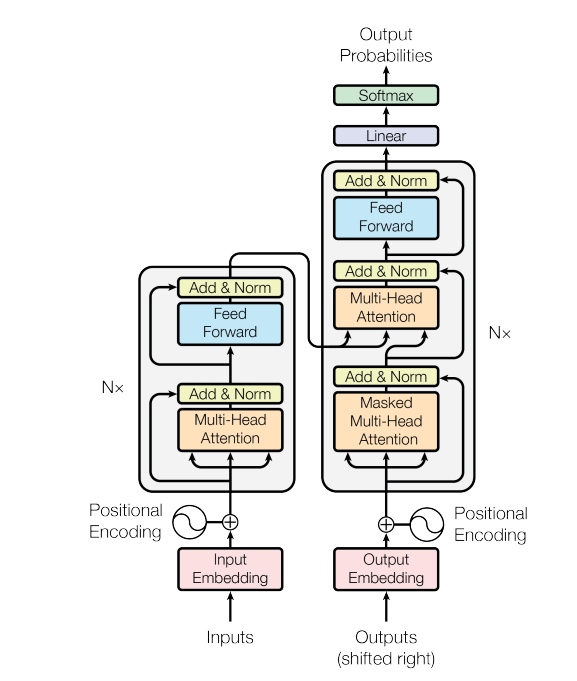
\includegraphics[scale=0.9]{images/Transformers.png}
\end{center}
\section{Input Embedding}
An embedding is a vector that \textbf{semantically} represents an object/input. In the context of NLP, the goal is to transform a text (set of words) into a vector of numbers such that similar words produce similar vectors. The \textbf{word2vec} technique is based on a feed-forward, fully connected architecture. It is similar to an autoencoder, but rather than performing input reconstruction, word2vec trains words according to other words that are neighbors in the input corpus.
\newline\newline
Word2vec can learn word embedding in two different ways:
\begin{itemize}
    \item \textbf{CBOW} (Continuous Bag of Words) in which the neural network uses the context to predict a target word.

    \item \textbf{Skip-gram} in which it uses the target word to predict a target context.
\end{itemize}
\begin{center}
    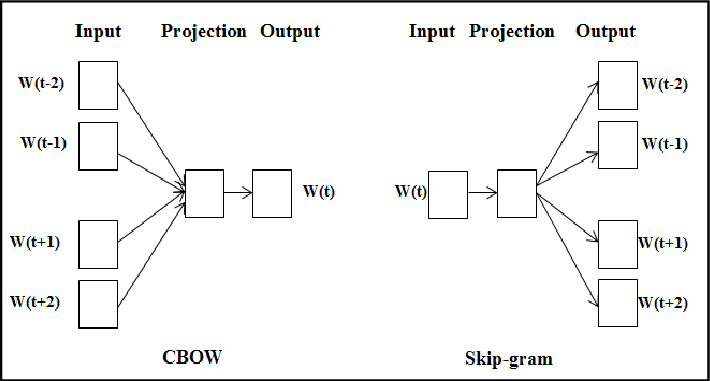
\includegraphics[scale = 0.4]{images/word2vec.png}
\end{center}


\section{Positional Encoding}
Position and order of words are the essential parts of any language. They define the grammar and thus the actual semantics of a sentence. Recurrent Neural Networks (RNNs) inherently take the order of word into account. They parse a sentence word by word in a sequential manner. This will integrate the words’ order in the backbone of RNNs.
\newline\newline
Since the model contains no recurrence and no convolution, in order for the model to make use of the order of the sequence, we must inject some information about the relative or absolute position of the tokens in the sequence.\newline\newline
One possible solution to give the model some sense of order is the \textbf{positional encoding}.\newline\newline
Positional encoding describes the location or position of an entity in a sequence so that each position is assigned a unique representation. There are many reasons why a single number, such as the index value, is not used to represent an item’s position in transformer models. For long sequences, the indices can grow large in magnitude. If you normalize the index value to lie between 0 and 1, it can create problems for variable length sequences as they would be normalized differently.\newline\newline
Transformers use a smart positional encoding scheme, where each position/index is mapped to a vector. Hence, the output of the positional encoding layer is a matrix, where each row of the matrix represents an encoded object of the sequence summed with its positional information.\newline\newline
Suppose you have an input sequence of length $L$. The positional encoding is given by sine and cosine functions of varying frequencies:
\[
\begin{split}
    PE_{(k, 2i)} & = sin(k/n^{2i/d})\\
    PE_{(k, 2i + 1)} & = cos(k/n^{2i/d})
\end{split}
\]
where:
\begin{itemize}
    \item $k$ is the position of an object in the input sequence.
    \item $d$ is the dimension of the output embedding space.
    \item $PE_{(k,j)}$ is the position function for mapping a position $k$ in the input sequence to index $j$ of the positional matrix.
    \item $n$ is a user-defined scalar, set to 10000 by the authors of the original Transformer's paper.
    \item $i$ is used for mapping to column indices $ 0 \leq i < d/2$, with a single value of $i$ maps to \textbf{both} sine and cosine functions.
\end{itemize}
You can also imagine the positional embedding as a vector containing pairs of sines and cosines for each frequency.
\begin{center}
    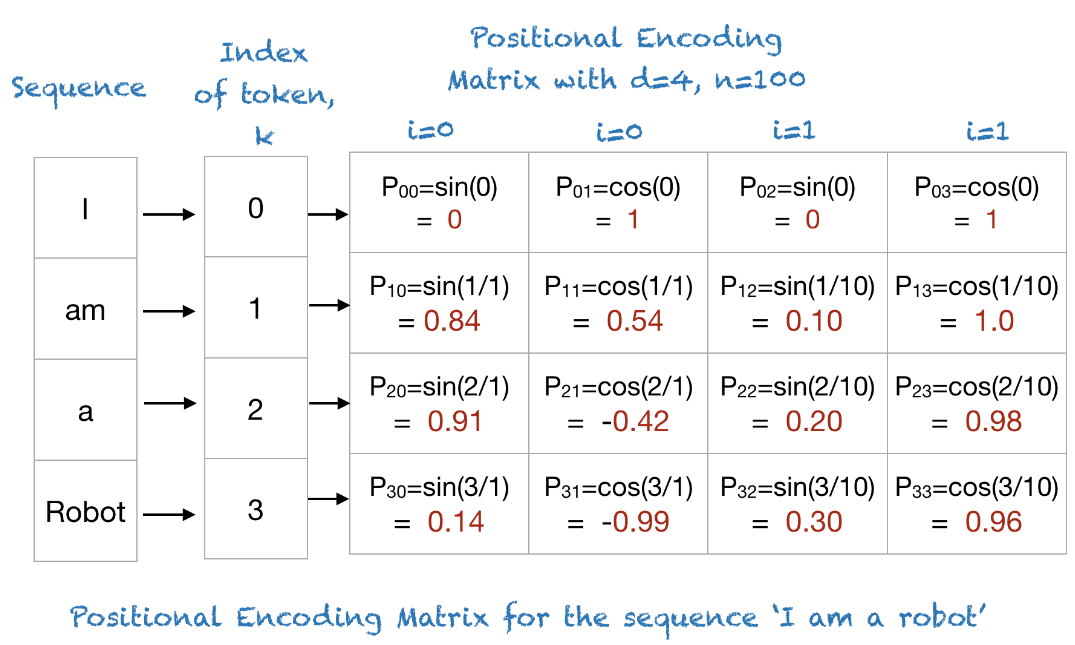
\includegraphics[scale=0.6]{images/Positional encoding.png}
\end{center}
The scheme for positional encoding has a number of advantages:
\begin{itemize}
    \item The sine and cosine functions have values in $[-1, 1]$, which keeps the values of the positional encoding matrix in a normalized range.

    \item As the sinusoid for each position is different, you have a unique way of encoding each position.

    \item You have a way to add positional information to words embedding in order to encode the relative positions of words (e.g. the words 'brother' and 'sister' will probably have similar embedding representations, but if one word is used in a very different position than the other, they may not be correlated. In order to get different representations, we add positional information). 
\end{itemize}
The positional encoding layer sums the positional vector with corresponding word embedding vector.
\begin{center}
    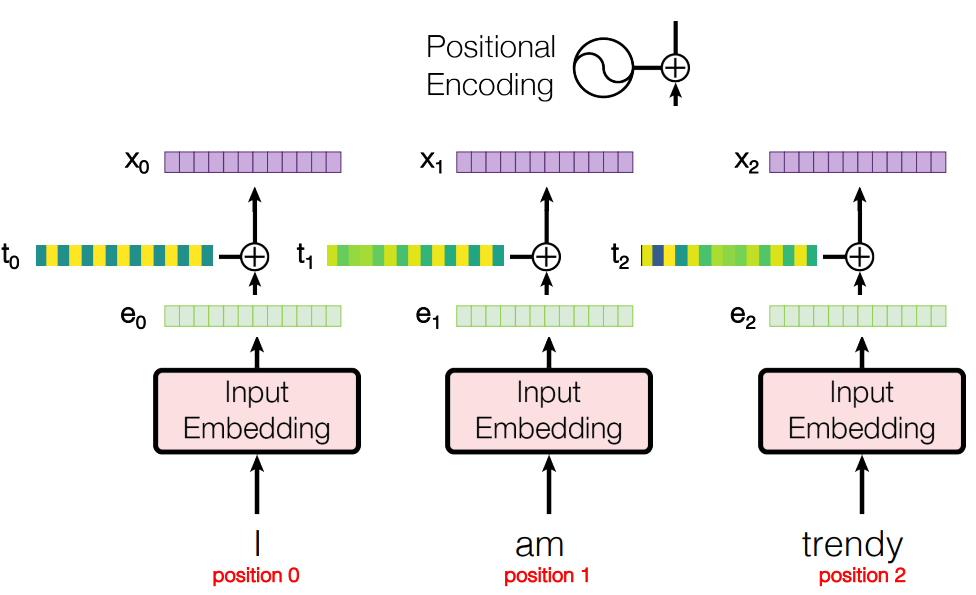
\includegraphics[scale=0.6]{images/positional encoding 2.png}
\end{center}

\section{Attention}
In order for the decoding to be precise, it needs to take into account every word of the input, using attention.\newline\newline
An attention function can be described as mapping a query and a set of key-value pairs to an output, where the query, keys, values, and output are all vectors. The output is computed as a weighted sum of the values, where the weight assigned to each value is computed by a compatibility function of the query with the corresponding key.
\begin{center}
    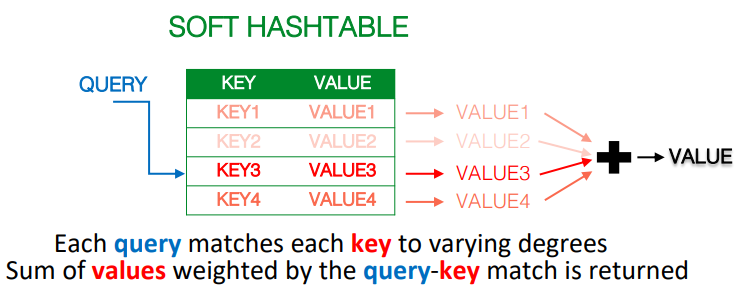
\includegraphics[scale=0.8]{images/attention.png}
\end{center}
The first step in calculating attention is to create three vectors from each of the encoder’s input vectors. So for each word, we create a \textbf{Query vector}, a \textbf{Key vector}, and a \textbf{Value vector}. These vectors are created by multiplying the embedding by three matrices ($\textbf{W}^\textbf{Q}, \textbf{W}^\textbf{K}, \textbf{W}^\textbf{V}$) that we trained during the training process.
\begin{center}
    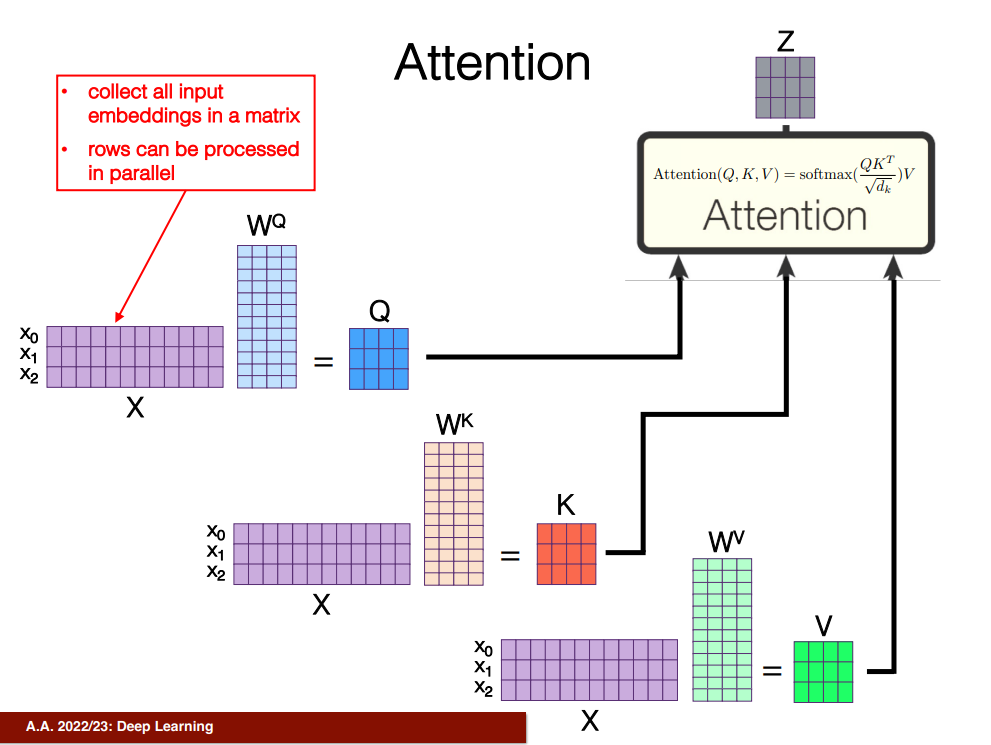
\includegraphics[scale=0.6]{images/attention 2.png}
\end{center}
If we collect all the query, keys and value vectors in three matrices ($\textbf{Q}, \textbf{K}, \textbf{V}$), we can define the attention function as follows:
\[\text{Attention}(Q,K,V) = \text{softmax}\left(\frac{QK^T}{\sqrt{d_k}}\right)V\]
By taking the dot product between the query matrix and the key matrix, we compute a \textit{score} for each word of the input sentence against the others. The score determines how relevant is a word with respect to the others. The dot-products of queries and keys are divided by $\sqrt{d_k}$ (dimensionality of the embedding vector) to alleviate gradient vanishing problem of the softmax function. The softmax normalizes the scores so they’re all positive and add up to 1. $\text{softmax}\left(\frac{QK^T}{\sqrt{d_k}}\right)$ is often called \textbf{attention matrix}.\newline\newline
Then, we compute the dot product between the attention matrix and the value matrix $\textbf{V}$. The intuition here is to keep intact the values of the relevant word(s), and drown-out irrelevant words (by multiplying them by tiny numbers in the attention matrix).

\subsection{Multi-Head Attention}
Instead of simply applying a single attention function, Transformer uses \textbf{multi-head attention}, where queries keys and values are linearly projected $h$ times  with different, learned linear projections to $d_k$, $d_k$ and $d_v$ dimensions, respectively. On each of these projected versions of queries, keys and values we then perform the attention function in parallel, yielding $d_v$-dimensional output values. These are concatenated and once again projected, resulting in the final values.\newline\newline
Multi-head attention allows the model to jointly attend to information from different representation subspaces at different positions.
\[\text{MultiHead}(Q, K, V ) = \text{Concat}(head_1, ..., head_h)\textbf{W}^\textbf{O}\]
where
\[head_i = Attention(\textbf{Q}\textbf{W}_i^\textbf{Q}, \textbf{K}\textbf{W}_i^\textbf{K}, \textbf{V}\textbf{W}_i^\textbf{V})\]
\begin{center}
    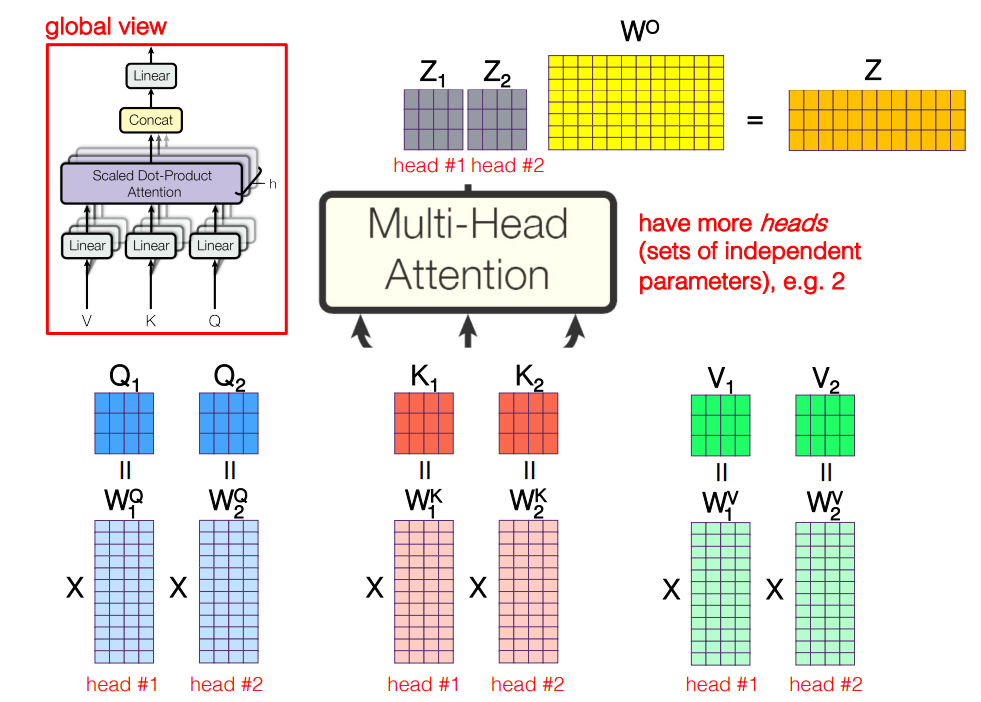
\includegraphics[scale=0.6]{images/multi-head attention.png}
\end{center}

\subsection{Applications of Attention in the Model}
The Transformer uses multi-head attention in three different ways:
\begin{itemize}
    \item In "encoder-decoder attention" layers (cross-attention), the queries come from the previous decoder layer, and the memory keys and values come from the output of the encoder. This allows every position in the decoder to attend over all positions in the input sequence. 

    \item The encoder contains \textbf{self-attention} layers. In a self-attention layer all of the keys, values and queries come from the same place, in this case, the output of the previous layer in the encoder stack. we set $\textbf{Q} = \textbf{K} = \textbf{V} = \textbf{Z}$, where $\textbf{Z}$ is the output of the previous encoder layer.

    \item Masked Self-attention: We need to prevent leftward information flow in the decoder to preserve the auto-regressive property. Therefore, in the Transformer decoder, the self-attention is restricted such that queries at each position can only attend to all key-value pairs up to and including that position. This is implemented inside of scaled dot-product attention by masking out (setting to $-\infty$) all values in the input of the softmax which correspond to illegal connections.
\end{itemize}

\section{Add \& Norm and Feed Forward Network}
In addition to attention sub-layers, each of the layers in the encoder and decoder contains a fully connected feed-forward network, which is applied to each position separately and identically. This consists of two linear transformations with a ReLU activation in between.
\[FFN(h) = max(0, hW_1 + b_1)W_2 + b_2\]
where $h$ is the output of the previous layer.\newline\newline
In order to build a deep model, Transformer employs a residual connection around each module, followed by Layer Normalization. For instance, each Transformer encoder block may be written as
\[\begin{split}
    \textbf{H'} & = \text{LayerNorm}(\text{SelfAttention(\textbf{X}) + \textbf{X}})\\
    \textbf{H} & = \text{LayerNorm}(FFN(\textbf{H'}) + \textbf{H'})    
\end{split}
\]
\begin{center}
    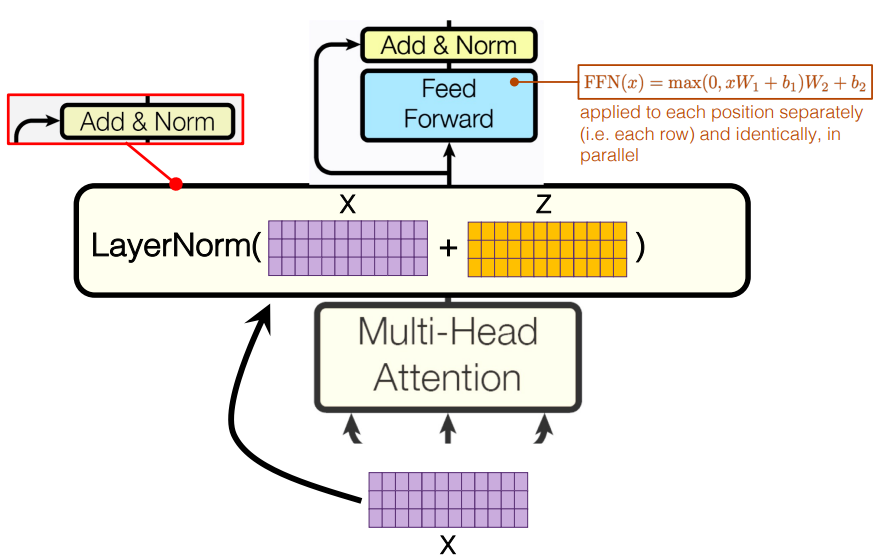
\includegraphics[scale=0.6]{images/LayerNorm.png}
\end{center}
